\chapter{Introduction} \label{chap:intro}

%%\section{Motivation}\label{sect:thefirst}
%\begin{itemize}
%    \item The use of the RGB-D camera, the use of depth information, application: visual odometry on quadcopter, human motion capture, 3D reconstruction.
%    \item but the depth image from consumer RGB-D camera has bad accuracy and noisy and missing data. does not contain any fine details, for example the button on the shirt, some wrincles on your hand, etc.
%        
%    it has been shown that with the noisy and imperfect measurements, the quality of the 3D reconstruction and the estimation of trajectory subject to. And these errors may accumulate frame by frame, leads to drift. and finally causes a loss of quality
%    \item some method tried to recover these details by fusing the depth data from multiple views~\cite{newcombe2011kinectfusion}, however, still the recovered details is very limited.
%    \item so here comes our work, we explore the intrinsic details of the object in an image, analyze the lights' positions and its corresponding influence of the shading on the object, the reflectance rate of the material on the objects.
%    \item talk a bit about SFS and PS, their basic definition: obtain the shape from an image when the light is known. 
%    \item say that combine SFS or PS with observed depth can eliminate ambiguities and has been widely used for shape or depth refinement by  and it is usually formulated as an inverse problem. and nonlinearity within the normal exists in such an inverse problem, some people tries to use some nonlinear optimization to solve this problems but makes the process super slow, some others freeze the nonlinear part with the thing in the last iteration, but this sometimes leads to divergence problem. So we have a good method.
%  
%    \item say that some state-of-the-art methods need to make some strict assumptions like constant albedo, but not really in line with real world objects. Some others try to estimate the albedo by imposing some piece-wise smoothness terms, but the estimation is not satisfying and the surface normal cannot be separated from the albedo. And here comes another new methods, and how good is ours
%    \item the idea of our two methods. use what as the input, first estimate waht, then waht then what. {\color{red}(we explicitly estimate the incident illumination in the scene based on the reconstructed shape, make an estimate of the albedo distribution on the surface, and then use this information together with the lighting equation to recover the fine-grained structure and orientation of points on the surface. We assume a Lam- bertian model of reflection where incident lighting is given by an environment map that is parameterized in the spher- ical harmonic domain, and where surface properties are given by a spatially-varying albedo map.)}
%\end{itemize}

\section{Motivation}
With the advent of affordable RGB-D cameras, many research areas in modern computer vision, computer graphics and robotics have been boosted significantly, such as 3D modelling and reconstruction, human motion capture and visual SLAM, etc.
Although the RGB-D sensors can return the depth information in addition to the RGB image, the depth quality is not satisfying.

\begin{figure}[!ht]
    \centering
    \subfigure[RGB image]{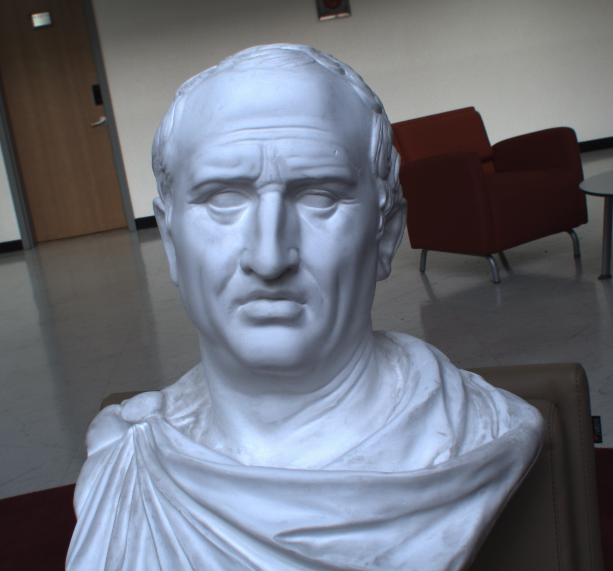
\includegraphics[width=0.28\linewidth]{figures/cicero_rgb.png}}
    \subfigure[Input depth]{\label{fig:cicero_input}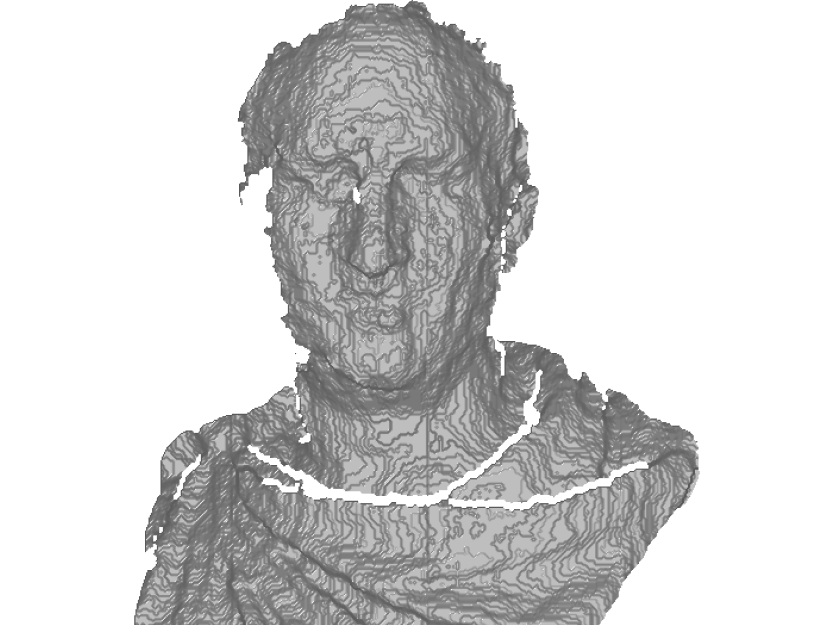
\includegraphics[width=0.32\linewidth]{figures/cicero_shape_init.pdf}}
    \subfigure[Refined depth with our RGBD-Fusion Like method]{\label{fig:cicero_output} 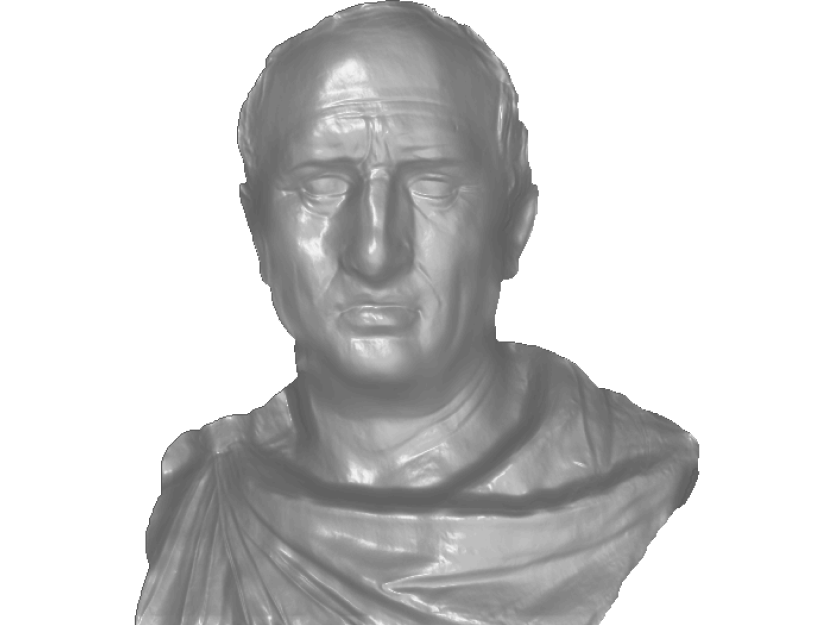
\includegraphics[width=0.32\linewidth]{figures/cicero_shape.pdf}}
    \caption{Illustrations for the task of depth refinement. The depths are plotted as a surface for the sake of a better visualization. The RGB-D data is taken by Kinect~\cite{han2013high}.}
    \label{fig:intro_illu}
\end{figure}


As we can notice from Fig.~\ref{fig:cicero_input}, the depth map is very noisy, on which many regions also have missing depth values.
What's more, there are no many fine details on the rough depth.
It has been shown that the quality of 3D reconstruction of an object may suffer from the noisy and imperfect depth measurements, and the estimation of camera trajectory will also drift severely because of the accumulated errors on the depths.
There are some methods trying to recover these details by fusing all the depth data from multiple views~\cite{newcombe2011kinectfusion}, nevertheless, the recovered details are still very limited.
Provided we can improve the quality of input rough depth in Fig.~\ref{fig:cicero_input} to the refined depth in Fig.~\ref{fig:cicero_output}, all the tasks which are relied on RGB-D sensors can be made considerable progress. 

\section{Problem statement}

In this dissertation, we delve into the research of the refinement of a single depth map.
To refine the depth information from consumer depth sensors, the intrinsic details of an object should be explored with the aid of RGB image(s).
The analyzation includes the positions of the scene illuminations and their corresponding influences in the shading on the object, and also the reflectance (albedo) of the object's material.
Shape from shading (SFS) and photometric stereo (PS) are the approaches which can study the intrinsic properties of images, so they have been successfully integrated with many state-of-the-art depth enhancement methods.
These shading-based methods can be formulated with the Lambertian reflectance model in which nonlinearity exists. 
Some methods~\cite{wu2014real, or2016real} directly apply the nonlinear optimization algorithm like Levenberg-Marquardt or ADMM scheme to solve the problem which leads to the runtime issue. 
Other methods like~\cite{or2015rgbd} freeze the nonlinear part with the outcome from the last iteration, so the nonlinearity has been cancelled out.
However, such fixed-point scheme sometimes causes the optimization divergent.
Therefore, we propose a method called RGB ratio model.
With the red, green and blue LED lights set up in various directions, we are able to build a lighting model for each channel of the color image acquired from RGB-D sensors.
The proposed setup and model could resolve the nonlinearity and have a closed-form solution. 
It will be shown in chapter~\ref{chap:result} that the RGB ratio model achieves similar accuracy to the state-of-the-art methods, while even have better performance in some cases.


Also, it should be mentioned that many shading-based depth refinement methods require making the assumption that the albedo is either uniform or constant, and others impose some piecewise smoothness constraints on the albedo to make this inverse problem well-posed.
These methods work well on some uncomplicated objects, for example, the statue in Fig.~\ref{fig:intro_illu}, but have the difficulty to separate the changes in the albedo from the shape when the albedo becomes complex.
It is indeed reasonable because numerous real-world objects have rather complicated patterns and colors.
Consequently, we present another novel approach called robust multi-light method which can handle the case of very complicated albedos.
The idea is to acquire several images from various illuminations with the fixed camera view, and use all the information to jointly refine the light, albedo and depth iteratively.
To simulate the scenario of multiple lighting conditions, we sway a white LED light source (could be the phone flashlight) and consistently capture images. 
Compared to other methods, one another main advantage of the proposed method is not any regularization terms need to be imposed, which saves a number of unpredictable time for tedious parameter tuning process.

Last but not the least, since the depth maps acquired from consumer RGB-D sensors usually do not have the satisfying resolution, we use the higher-resolution RGB images and have managed to integrate image super-resolution with our depth refinement method.
In this way, the final refined depth can attain the same resolution as the large RGB images with all the fine details.
We believe this is the first shading-based depth super-resolution approach.

The main contributions of this dissertation are:
\begin{enumerate}
    \item We present a more efficient and faster implementation of an advanced depth refinement method~\cite{or2015rgbd}.
    \item We propose a new RGB ratio model to resolve the nonlinearity and achieve similar accuracy to the state-of-the-art methods.
    \item We introduce a robust multi-light method which outperforms the other depth refinement approaches both quantitatively and qualitatively. Moreover, no regularization is imposed at all.
    \item We combine the image super-resolution with our method and present the high-quality and high-resolution depth.
\end{enumerate}


\section{Outline}
The outline of this thesis is structured as follows:

Have not finished yet.
